% ================================================================
% figs-batch2.tex —— 第 2 批手绘示意图的 TikZ 重绘（15 幅图体）
% 覆盖 p.51（2 幅）、p.52、p.63、p.65、p.77、p.85、p.97（2 幅）、
%      p.106、p.107、p.120、p.121（2 幅）、p.122。
% 只含图体：不含 figure 环境与 caption，不引用外部图片，不写
% \usepackage、\usetikzlibrary（假定已装载 arrows.meta, calc,
% decorations.pathmorphing, patterns）。
% 命名 figP<页>[A|B]。控制序列名不能含数字，故用 \csname 定义；
% 正文写 \figP{051A}、\figP{121B}（文件末有转发宏）。
% p.121 的 X^+ / X^- 原文并排为同一幅图，也可分开使用。
% ================================================================

% p.51：$|\Bun_1|=|\mathrm{Pic}|\cong\mathbb Z$ 离散，点是 $\mathcal O(i)$（例 10.6）
\expandafter\newcommand\csname figP051A\endcsname{%
\begin{tikzpicture}[scale=0.9]
  \node[left] at (-0.3,0) {$|\Bun_1|$};
  \foreach \y/\l in {2.0/{$\mathcal O(2)$},1.0/{$\mathcal O(1)$},0/{$0$},
                     -1.0/{$\mathcal O(-1)$},-2.0/{$\mathcal O(-2)$}}{%
    \fill (0.6,\y) circle (1.5pt);
    \node[right] at (0.8,\y) {\small \l};}
  \node at (0.6,2.75) {$\vdots$};
  \node at (0.6,-2.75) {$\vdots$};
\end{tikzpicture}}

% p.51：$|\Bun_2|$ 按次数 $d$ 分层，每层唯一半稳定点 $\mathcal O(d/2)$；
% 红色波浪箭头是特化，向右越来越特殊（例 10.7，$\otimes\mathcal O(1)$ 使其 2-周期）
\expandafter\newcommand\csname figP051B\endcsname{%
\begin{tikzpicture}[scale=0.9,
  sp/.style={red,decorate,decoration={snake,amplitude=0.9pt,segment length=4pt}}]
  \node[left] at (-0.5,0.2) {$|\Bun_2|$};
  \foreach \y/\d in {2.9/{$d=1$},0.2/{$d=0$},-2.5/{$d=-1$}}
    \node[right] at (-0.4,\y) {\small \d};
  \foreach \y in {2.9,0.2,-2.5}{%
    \fill (1.6,\y) circle (2.4pt);
    \fill (4.3,\y) circle (1.4pt);
    \fill (6.9,\y) circle (1.4pt);
    \draw[sp,-{Stealth[length=3.5pt]}] (1.95,\y) -- (3.95,\y);
    \draw[sp,-{Stealth[length=3.5pt]}] (4.65,\y) -- (6.55,\y);}
  \node[above] at (1.45,3.15) {\scriptsize $\mathcal O(\tfrac12)$};
  \node[above] at (4.3,3.15) {\scriptsize $\mathcal O\oplus\mathcal O(1)$};
  \node[above] at (7.05,3.15) {\scriptsize $\mathcal O(-1)\oplus\mathcal O(2)$};
  \node[above] at (1.45,0.45) {\scriptsize $\mathcal O^2$};
  \node[above] at (4.3,0.45) {\scriptsize $\mathcal O(-1)\oplus\mathcal O(1)$};
  \node[above] at (7.05,0.45) {\scriptsize $\mathcal O(-2)\oplus\mathcal O(2)$};
  \node[above] at (1.45,-2.25) {\scriptsize $\mathcal O(-\tfrac12)$};
  \node[above] at (4.3,-2.25) {\scriptsize $\mathcal O(-1)\oplus\mathcal O$};
  \node[above] at (7.05,-2.25) {\scriptsize $\mathcal O(-2)\oplus\mathcal O(1)$};
  \node[red] at (4.3,-3.5) {\scriptsize specializations};
\end{tikzpicture}}

% p.52：$|\Bun_3|$ 的 $d=0$ 层开头——$\mathcal O^3$ 特化到两个半稳定点，
% 二者又同样特化到 $\mathcal O(-1)\oplus\mathcal O\oplus\mathcal O(1)$（例 10.8）
\expandafter\newcommand\csname figP052\endcsname{%
\begin{tikzpicture}[scale=0.9,
  sp/.style={red,decorate,decoration={snake,amplitude=0.9pt,segment length=4pt}}]
  \node[left] at (-1.0,0.6) {$|\Bun_3|$};
  \node[left] at (-1.0,-0.2) {\small $d=0$};
  \fill (0,0) circle (2.4pt);
  \node[below left] at (-0.15,-0.2) {\small $\mathcal O^3$};
  \fill (2.6,2.0) circle (1.5pt);
  \fill (2.6,-2.0) circle (1.5pt);
  \fill (5.2,0.35) circle (1.5pt);
  \node[above] at (2.6,2.25) {\scriptsize $\mathcal O(-\tfrac12)\oplus\mathcal O(1)$};
  \node[below] at (2.6,-2.25) {\scriptsize $\mathcal O(-1)\oplus\mathcal O(\tfrac12)$};
  \node[below right] at (5.05,0.0) {\scriptsize $\mathcal O(-1)\oplus\mathcal O\oplus\mathcal O(1)$};
  \draw[sp,-{Stealth[length=3.5pt]}] (0.35,0.3) -- (2.25,1.78);
  \draw[sp,-{Stealth[length=3.5pt]}] (0.35,-0.3) -- (2.25,-1.78);
  \draw[sp,-{Stealth[length=3.5pt]}] (2.95,1.8) -- (4.9,0.6);
  \draw[sp,-{Stealth[length=3.5pt]}] (2.95,-1.8) -- (4.9,-0.6);
  \node at (7.6,2.05) {$\cdots$};
  \node at (7.6,-2.05) {$\cdots$};
\end{tikzpicture}}

% p.63：$R$ 的“单参数形变”。底部是 $\Spa R^\flat$，四条竖线是 $\xi$-方向纤维，
% 横穿的黑曲线 $\xi_R=\Spa W_{\mathcal O_E}(R^{\flat\circ})\setminus V([\![\varpi]\!])$
% 上的红带子是 $B^+_{dR}$ 部分（§12.3）
\expandafter\newcommand\csname figP063\endcsname{%
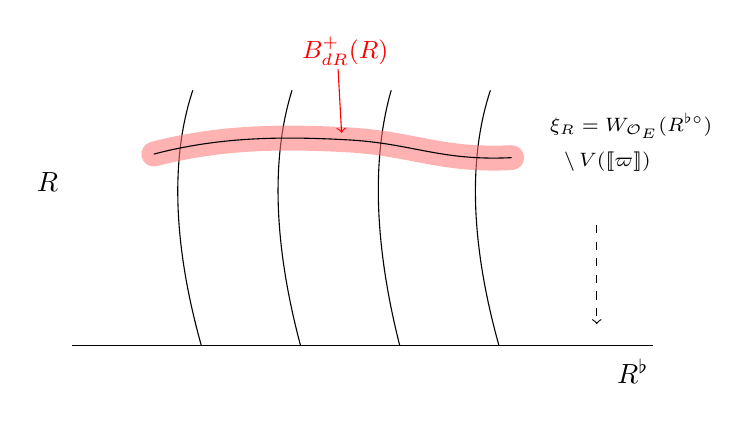
\begin{tikzpicture}[scale=0.9]
  \draw (-0.6,0) -- (7.6,0);
  \foreach \x/\d in {1.1/-0.30,2.5/-0.28,3.9/-0.26,5.3/-0.30}
    \draw (\x,3.6) .. controls (\x+\d,2.7) and (\x+\d,1.5) .. (\x+0.12,0);
  \draw[red!55,line width=9pt,opacity=0.55,line cap=round]
        (0.55,2.7) .. controls (1.5,2.95) and (2.4,2.95) .. (3.3,2.9)
        .. controls (4.2,2.85) and (4.6,2.6) .. (5.6,2.65);
  \draw (0.55,2.7) .. controls (1.5,2.95) and (2.4,2.95) .. (3.3,2.9)
        .. controls (4.2,2.85) and (4.6,2.6) .. (5.6,2.65);
  \node[red] at (3.25,4.15) {\small $B^+_{dR}(R)$};
  \draw[->,red] (3.15,3.9) -- (3.2,3.0);
  \node at (-0.95,2.3) {$\Spa R$};
  \node[anchor=west] at (6.0,3.1) {\scriptsize $\xi_R=\Spa W_{\mathcal O_E}(R^{\flat\circ})$};
  \node[anchor=west] at (6.2,2.6) {\scriptsize $\setminus\,V([\![\varpi]\!])$};
  \draw[->,dashed] (6.8,1.7) -- (6.8,0.3);
  \node[below right] at (6.95,-0.05) {$\Spa R^\flat$};
\end{tikzpicture}}

% p.65：代数曲线 $X^{\mathrm{alg}}_{S^\flat}$ 上的点 $s$ 对应 $\Spa B^+_{dR}(R)$，
% 即 $\mathcal E'|_{X_s}$ 的局部模型（定理 12.25 证明）
\expandafter\newcommand\csname figP065\endcsname{%
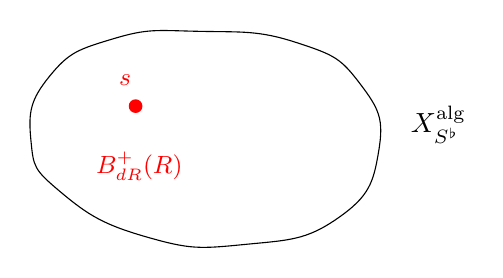
\begin{tikzpicture}[scale=0.95]
  \draw plot[smooth cycle,tension=0.85] coordinates
    {(-2.45,0.1) (-2.2,0.95) (-1.35,1.45) (-0.2,1.55) (1.1,1.4) (1.95,0.85)
     (2.2,-0.05) (1.65,-0.95) (0.4,-1.3) (-0.9,-1.2) (-2.05,-0.6)};
  \fill[red] (-1.05,0.55) circle (2.6pt);
  \node[red,above left] at (-0.98,0.7) {\small $s$};
  \node[red] at (-1.0,-0.25) {\small $B^+_{dR}(R)$};
  \node[right] at (2.5,0.3) {$X^{\mathrm{alg}}_{S^\flat}$};
\end{tikzpicture}}

% p.77：$\mathbb B_C$（左）、$\mathbb P^1_C$（右）、典范紧化
% $\overline{\mathbb B}^{\,/C}_C$（下）；紧化只多加一个“半径 $1$ 再加无穷小”的
% rank 2 点（例 14.12）。虚线弧表示树在无穷处继续
\expandafter\newcommand\csname figP077\endcsname{%
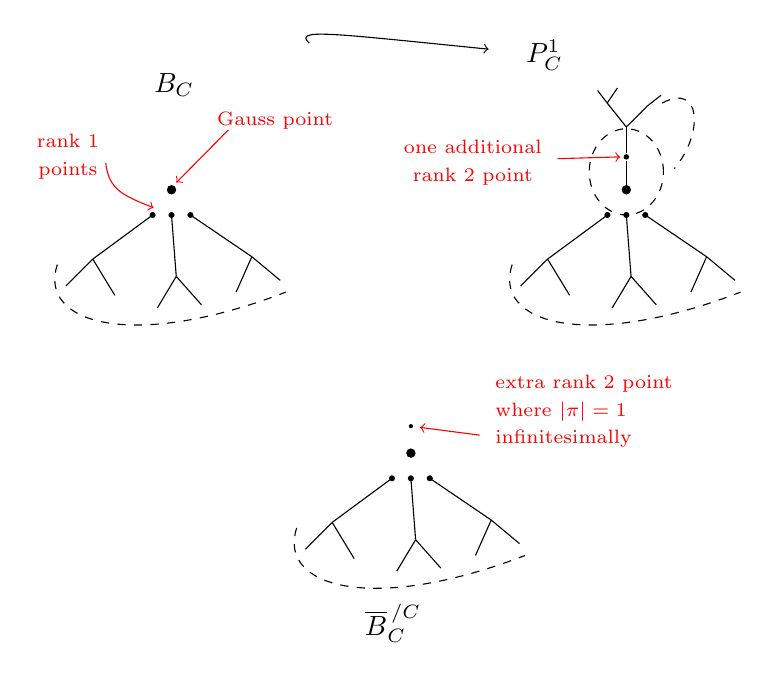
\begin{tikzpicture}[scale=0.76,
  tree/.pic={\fill (0,0) circle (1.7pt);
    \foreach \a in {-0.24,0,0.24} \fill (\a,-0.32) circle (1.1pt);
    \draw (-0.24,-0.32) -- (-1.00,-0.88) (0,-0.32) -- (0.06,-1.10)
          (0.24,-0.32) -- (1.02,-0.85);
    \draw (-1.00,-0.88) -- (-1.34,-1.22) (-1.00,-0.88) -- (-0.72,-1.34);
    \draw (0.06,-1.10) -- (-0.18,-1.50) (0.06,-1.10) -- (0.38,-1.46);
    \draw (1.02,-0.85) -- (0.82,-1.30) (1.02,-0.85) -- (1.38,-1.15);
    \draw[dashed] (-1.45,-0.95) .. controls (-1.70,-1.70) and (-0.50,-2.05) .. (1.45,-1.30);}]
  \pic at (0,0) {tree};
  \node[anchor=west] at (-0.45,1.75) {$\mathbb B_C$};
  \node[red,anchor=west] at (0.60,1.15) {\scriptsize Gauss point};
  \draw[->,red] (0.95,1.00) -- (0.08,0.12);
  \node[red,align=center,anchor=east] at (-1.05,0.55)
    {\scriptsize rank 1\\[-2pt]\scriptsize points};
  \draw[->,red] (-1.10,0.45) .. controls (-1.05,0.0) and (-0.80,-0.10) .. (-0.30,-0.30);
  \draw[->] (2.3,2.45) .. controls (2.05,2.70) and (2.6,2.62) .. (5.3,2.35);
  \pic at (7.6,0) {tree};
  \draw (7.6,0) -- (7.6,0.48);
  \fill (7.6,0.55) circle (1.3pt);
  \draw (7.6,0.62) -- (7.6,1.05);
  \draw (7.6,1.05) -- (7.28,1.45) (7.6,1.05) -- (7.95,1.40);
  \draw (7.28,1.45) -- (7.12,1.66) (7.28,1.45) -- (7.45,1.70);
  \draw (7.95,1.40) -- (8.18,1.58);
  \draw[dashed] (7.6,0.30) ellipse (0.62 and 0.72);
  \draw[dashed] (8.20,1.45) .. controls (8.85,1.80) and (8.90,0.95) .. (8.40,0.35);
  \node[red,align=center,anchor=east] at (6.35,0.45)
    {\scriptsize one additional\\[-2pt]\scriptsize rank 2 point};
  \draw[->,red] (6.45,0.52) -- (7.50,0.55);
  \node[anchor=east] at (6.70,2.25) {$\mathbb P^1_C$};
  \pic at (4.0,-4.4) {tree};
  \fill (4.0,-3.95) circle (1.0pt);
  \draw[->,red] (5.15,-4.10) -- (4.15,-3.97);
  \node[red,align=left,anchor=west] at (5.25,-3.70)
    {\scriptsize extra rank 2 point\\[-2pt]\scriptsize where $|\pi|=1$\\[-2pt]\scriptsize infinitesimally};
  \node[anchor=north] at (3.70,-6.75) {$\overline{\mathbb B}^{\,/C}_C$};
\end{tikzpicture}}

% p.85：$|\Bun_G|$ 一条连通分支内的特化图景：每层的点都特化到更特殊的点，
% 一路到底即半稳定层 $\Bun^{ss}_G$（推论 16.2：连通分支 = 某半稳定层的闭包）
\expandafter\newcommand\csname figP085\endcsname{%
\begin{tikzpicture}[scale=1.1,
  sp/.style={red,decorate,decoration={snake,amplitude=0.9pt,segment length=4pt}}]
  \foreach \x in {1.0,2.0} \fill ( \x,3.7) circle (2.2pt);
  \fill (3.6,3.7) circle (2.6pt);
  \fill (5.2,3.7) circle (4.2pt);
  \draw[sp,-{Stealth[length=3.5pt]}] (4.8,3.7) -- (4.0,3.7);
  \draw[sp,-{Stealth[length=3.5pt]}] (3.3,3.8) -- (2.4,4.0);
  \draw[sp,-{Stealth[length=3.5pt]}] (3.3,3.6) -- (2.4,3.4);
  \draw[sp,-{Stealth[length=3.5pt]}] (1.8,4.0) -- (1.2,4.05);
  \draw[sp,-{Stealth[length=3.5pt]}] (1.8,3.4) -- (1.2,3.35);
  \fill (5.2,1.1) circle (4.2pt);
  \foreach \y in {1.75,1.1,0.45} \fill (3.6,\y) circle (2.6pt);
  \foreach \y in {1.95,1.1,0.25} \fill (2.0,\y) circle (2.6pt);
  \foreach \y in {1.75,1.1,0.45}
    \draw[sp,-{Stealth[length=3.5pt]}] (4.8,\y) -- (4.0,\y);
  \foreach \y/\z in {1.75/1.95,1.1/1.1,0.45/0.25}
    \draw[sp,-{Stealth[length=3.5pt]}] (3.3,\y) -- (2.4,\z);
  \foreach \x in {3.2,3.55,3.9} \fill[red] (\x,-1.2) circle (2.2pt);
  \fill (5.2,-1.2) circle (4.2pt);
  \foreach \y in {-1.9,-2.3,-2.7} \fill (5.2,\y) circle (1.6pt);
  \draw (4.5,-3.15) .. controls (4.75,-3.0) and (5.0,-3.3) .. (5.3,-3.1)
        .. controls (5.5,-2.95) and (5.7,-3.15) .. (5.8,-3.3);
  \node at (5.2,-3.85) {$\Bun^{ss}_G$};
  \draw[->] (5.9,3.7) -- (7.2,3.7);
  \node at (0.55,3.7) {$\cdots$};
  \node at (0.55,1.1) {$\cdots$};
\end{tikzpicture}}

% p.97：$|X_{\bar x}|$ 与 $|S_{\bar s}|$ 都是全序点链；$|S_{\bar t}|\subset|S_{\bar s}|$
% 是其中的子链（椭圆圈出），竖箭头是 $X_{\bar x}\to S_{\bar s}$（注 18.18）
\expandafter\newcommand\csname figP097A\endcsname{%
\begin{tikzpicture}[scale=0.9,
  sq/.style={decorate,decoration={snake,amplitude=1.0pt,segment length=3.6pt}}]
  \node[left] at (1.5,3.2) {$|X_{\bar x}|$};
  \fill (2.2,3.2) circle (3.2pt);
  \foreach \x in {3.4,4.6,5.9} \fill (\x,3.2) circle (1.7pt);
  \draw[sq,-{Stealth[length=3.5pt]}] (2.6,3.2) -- (3.1,3.2);
  \draw[sq,-{Stealth[length=3.5pt]}] (3.7,3.2) -- (4.3,3.2);
  \draw[sq,-{Stealth[length=3.5pt]}] (4.9,3.2) -- (5.55,3.2);
  \draw[->] (0.7,2.5) -- (0.7,1.1);
  \node[left] at (1.5,-0.3) {$|S_{\bar s}|$};
  \fill (2.2,-0.3) circle (3.2pt);
  \foreach \x in {3.4,4.6,5.8,7.0} \fill (\x,-0.3) circle (1.7pt);
  \draw[sq,-{Stealth[length=3.5pt]}] (2.6,-0.3) -- (3.1,-0.3);
  \draw[sq,-{Stealth[length=3.5pt]}] (3.7,-0.3) -- (4.3,-0.3);
  \draw[sq,-{Stealth[length=3.5pt]}] (4.9,-0.3) -- (5.5,-0.3);
  \draw[sq,-{Stealth[length=3.5pt]}] (6.1,-0.3) -- (6.7,-0.3);
  \draw (3.4,-0.3) ellipse (1.9 and 0.62);
  \node at (3.4,-1.25) {$|S_{\bar t}|$};
\end{tikzpicture}}

% p.97：过收敛（overconvergent）。把树上的点 $x$ 放大：黑块是点本身，
% 三个红点是它周围的 rank 1 点，四条短线是各个方向（注 18.18 之后的直观图）
\expandafter\newcommand\csname figP097B\endcsname{%
\begin{tikzpicture}[scale=0.9,
  tree/.pic={\fill (0,0) circle (1.6pt);
    \draw (0,0) -- (-0.95,-0.9) (0,0) -- (0.05,-1.1) (0,0) -- (0.98,-0.85);
    \draw (-0.95,-0.9) -- (-1.32,-1.25) (-0.95,-0.9) -- (-0.70,-1.38);
    \draw (0.05,-1.1) -- (-0.20,-1.55) (0.05,-1.1) -- (0.36,-1.50);
    \draw (0.98,-0.85) -- (0.80,-1.35) (0.98,-0.85) -- (1.38,-1.18);}]
  \pic at (0.8,-0.1) {tree};
  \draw[dashed] (0.8,-0.1) circle (0.72);
  \draw[->] (3.75,1.35) -- (1.62,0.55);
  \draw (5.9,1.1) circle (1.85);
  \fill[gray!12] (5.9,1.25) circle (1.05);
  \draw[gray] (5.9,1.25) circle (1.05);
  \fill (6.25,1.75) circle (0.34);
  \foreach \a in {150,20,-35} \fill[red] ($(6.0,1.3)+(\a:0.62)$) circle (0.055);
  \draw ($(6.0,1.0)+(200:0.75)$) -- ($(6.0,1.0)+(200:1.15)$);
  \draw ($(6.0,1.0)+(250:0.75)$) -- ($(6.0,1.0)+(250:1.15)$);
  \draw ($(6.0,1.0)+(300:0.75)$) -- ($(6.0,1.0)+(300:1.15)$);
  \draw ($(6.0,1.4)+(160:0.85)$) -- ($(6.0,1.4)+(160:1.20)$);
\end{tikzpicture}}

% p.106：$\tilde M_b\cong\mathcal{BC}(\mathcal O(-1)[1])$ 是开单位圆盘；中心是
% $t=0$，右上边界圈出被挖去的点 $*$——它在 $|t|=1$ 处（警告 19.16）
\expandafter\newcommand\csname figP106\endcsname{%
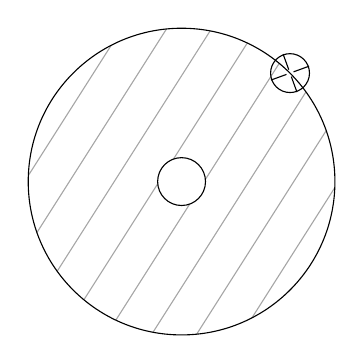
\begin{tikzpicture}[scale=0.95]
  \begin{scope}
    \clip (0,0) circle (2.05);
    \foreach \t in {-2.8,-2.2,...,2.8} \draw[gray!70] (\t-1.3,-2.2) -- (\t+1.5,2.2);
  \end{scope}
  \draw (0,0) circle (2.05);
  \fill[white] (0,0) circle (0.32);
  \draw (0,0) circle (0.32);
  \draw (1.45,1.45) circle (0.26);
  \foreach \a in {20,110,200,290}
    \draw (1.45,1.45) ++(\a:0.05) -- ++(\a:0.22);
\end{tikzpicture}}

% p.107：直观图——$M$ 带自由的 $\mathbb R$-作用（水平流线），$M/\mathbb R$ 紧
% （椭圆是截面），流的两个端点是“源”和“汇”（定理 19.19 的证明）
\expandafter\newcommand\csname figP107\endcsname{%
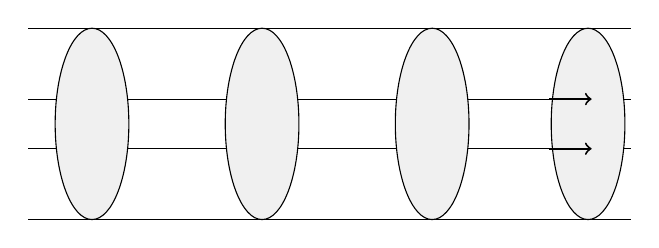
\begin{tikzpicture}[scale=0.9]
  \draw (0,2.85) -- (8.5,2.85);
  \draw (0,1.85) -- (8.5,1.85);
  \draw (0,1.15) -- (8.5,1.15);
  \draw (0,0.15) -- (8.5,0.15);
  \foreach \x in {0.9,3.3,5.7,7.9} \fill[gray!12] (\x,1.5) ellipse (0.52 and 1.35);
  \foreach \x in {0.9,3.3,5.7,7.9} \draw (\x,1.5) ellipse (0.52 and 1.35);
  \draw[->,line width=0.7pt] (7.35,1.85) -- (7.95,1.85);
  \draw[->,line width=0.7pt] (7.35,1.15) -- (7.95,1.15);
\end{tikzpicture}}

% p.120：树上的点及其放大（残余圆盘）。黑块是 rank 2 点、红点是 rank 1 点，
% 短线表示各方向——点的维数正是由此读出的（§22.3，例 22.15）
\expandafter\newcommand\csname figP120\endcsname{%
\begin{tikzpicture}[scale=0.9,
  tree/.pic={\fill (0,0) circle (1.6pt);
    \draw (0,0) -- (-0.95,-0.9) (0,0) -- (0.05,-1.1) (0,0) -- (0.98,-0.85);
    \draw (-0.95,-0.9) -- (-1.32,-1.25) (-0.95,-0.9) -- (-0.70,-1.38);
    \draw (0.05,-1.1) -- (-0.20,-1.55) (0.05,-1.1) -- (0.36,-1.50);
    \draw (0.98,-0.85) -- (0.80,-1.35) (0.98,-0.85) -- (1.38,-1.18);}]
  \fill[gray!25] (0.6,0.1) circle (0.75);
  \pic at (0.6,0.1) {tree};
  \draw[gray] (0.6,0.1) circle (0.75);
  \draw[->] (3.6,1.6) -- (1.55,0.75);
  \fill[gray!18] (6.4,1.2) circle (2.05);
  \draw (6.4,1.2) circle (2.05);
  \fill (6.95,1.95) circle (0.40);
  \foreach \a in {150,15,-40} \fill[red] ($(6.6,1.35)+(\a:0.65)$) circle (0.06);
  \draw ($(6.6,1.0)+(200:0.8)$) -- ($(6.6,1.0)+(200:1.25)$);
  \draw ($(6.6,1.0)+(250:0.8)$) -- ($(6.6,1.0)+(250:1.25)$);
  \draw ($(6.6,1.0)+(300:0.8)$) -- ($(6.6,1.0)+(300:1.25)$);
  \draw ($(6.6,1.5)+(155:0.95)$) -- ($(6.6,1.5)+(155:1.35)$);
\end{tikzpicture}}

% p.121：$\mathbb P^1$ 上的标准 $\mathbb G_m$-作用，分层 $X^+=\mathbb A^1\sqcup\{\infty\}$：
% 蓝色流线都汇向 $0$，赤道前半实线、后半虚线（例 22.17）
\expandafter\newcommand\csname figP121A\endcsname{%
\begin{tikzpicture}[scale=0.95]
  \fill[gray!12] (0,0) circle (1.65);
  \draw (0,0) circle (1.65);
  \draw[dashed] (1.65,0) arc[start angle=0,end angle=180,x radius=1.65,y radius=0.45];
  \draw (1.65,0) arc[start angle=0,end angle=-180,x radius=1.65,y radius=0.45];
  \foreach \a in {-0.25,-0.07,0.13,0.33}{
    \draw[blue,thick,-{Stealth[length=4.5pt]}]
      (\a,{1.47-2.1*\a*\a}) .. controls ({2.6*\a-0.55},{0.82-0.4*\a})
      and ({2.7*\a-0.45},{-0.6-0.4*\a}) .. ({2.2*\a-0.05},{-1.45+1.6*\a*\a});}
  \fill[blue] (0,1.65) circle (2pt);
  \fill[blue] (0,-1.65) circle (2pt);
  \node[blue,above] at (0,1.70) {\small $\infty$};
  \node[blue,below] at (0,-1.70) {\small $0$};
  \node[blue,left] at (-1.95,1.35) {\small $X^+$};
\end{tikzpicture}}

% p.121：同一球面的另一半——$X^-=\{0\}\sqcup(\mathbb A^1)^-$，红色流线都汇向 $\infty$
\expandafter\newcommand\csname figP121B\endcsname{%
\begin{tikzpicture}[scale=0.95]
  \fill[gray!12] (0,0) circle (1.65);
  \draw (0,0) circle (1.65);
  \draw[dashed] (1.65,0) arc[start angle=0,end angle=180,x radius=1.65,y radius=0.45];
  \draw (1.65,0) arc[start angle=0,end angle=-180,x radius=1.65,y radius=0.45];
  \foreach \a in {-0.33,-0.13,0.07,0.25}{
    \draw[red,thick,-{Stealth[length=4.5pt]}]
      ({2.2*\a-0.05},{-1.45+1.6*\a*\a}) .. controls ({2.7*\a-0.45},{-0.6-0.4*\a})
      and ({2.6*\a-0.55},{0.82-0.4*\a}) .. (\a,{1.47-2.1*\a*\a});}
  \fill[red] (0,1.65) circle (2pt);
  \fill[red] (0,-1.65) circle (2pt);
  \node[red,above] at (0,1.70) {\small $\infty$};
  \node[red,below] at (0,-1.70) {\small $0$};
  \node[red,left] at (-1.95,1.35) {\small $X^-$};
\end{tikzpicture}}

% p.122：例 22.20——$\mathbb G_m$ 在 $\mathbb A^2$ 上的双曲作用
% $t\cdot(a_1,a_2)=(t^{-1}a_1,ta_2)$ 的相图：沿 $x$-轴流出，沿 $y$-轴流入
\expandafter\newcommand\csname figP122\endcsname{%
\begin{tikzpicture}[scale=1.0,
  fl/.style={blue,thick,-{Stealth[length=4.5pt]}}]
  \draw (-3.1,0) -- (3.1,0);
  \draw (0,-2.6) -- (0,2.8);
  \foreach \x in {-2.6,-1.8} \draw[fl] (\x+0.5,0) -- (\x,0);
  \foreach \x in {1.3,2.0,2.65} \draw[fl] (\x-0.4,0) -- (\x,0);
  \draw[fl] (0,2.0) -- (0,1.5);
  \draw[fl] (0,-1.85) -- (0,-1.35);
  \foreach \s in {-1,1}{%
    \draw[fl] (0.25*\s,2.45) .. controls (1.0*\s,2.1) and (1.7*\s,1.6) .. (2.7*\s,0.9);
    \draw[blue,thick] (0.12*\s,1.75) .. controls (0.75*\s,1.55) and (1.25*\s,1.15) .. (1.9*\s,0.6);
    \draw[fl] (0.25*\s,-2.4) .. controls (1.0*\s,-2.05) and (1.7*\s,-1.55) .. (2.7*\s,-0.85);
    \draw[blue,thick] (0.12*\s,-1.7) .. controls (0.75*\s,-1.5) and (1.25*\s,-1.1) .. (1.9*\s,-0.55);}
\end{tikzpicture}}

% 转发宏：正文写 \figP{051A}、\figP{121B} 等（\providecommand 便于多批共存）
\providecommand{\figP}[1]{\csname figP#1\endcsname}
